\documentclass{article}

\usepackage{minted}
\usepackage{graphicx}
\usepackage{geometry}
\usepackage{amsmath}
\usepackage[final]{pdfpages} 


\geometry{hmargin=1.5cm,vmargin=1.5cm}


\newcommand{\IMG}[3]{
\begin{figure}[H]
\centering
\includegraphics[scale=#3]{img/#1}%
\caption{#2}%
\label{#1}%
\end{figure}

}

\newcommand{\Stats}{\subsection{Stats}}
\newcommand{\HRule}{\rule{\linewidth}{0.5mm}}

\begin{document}


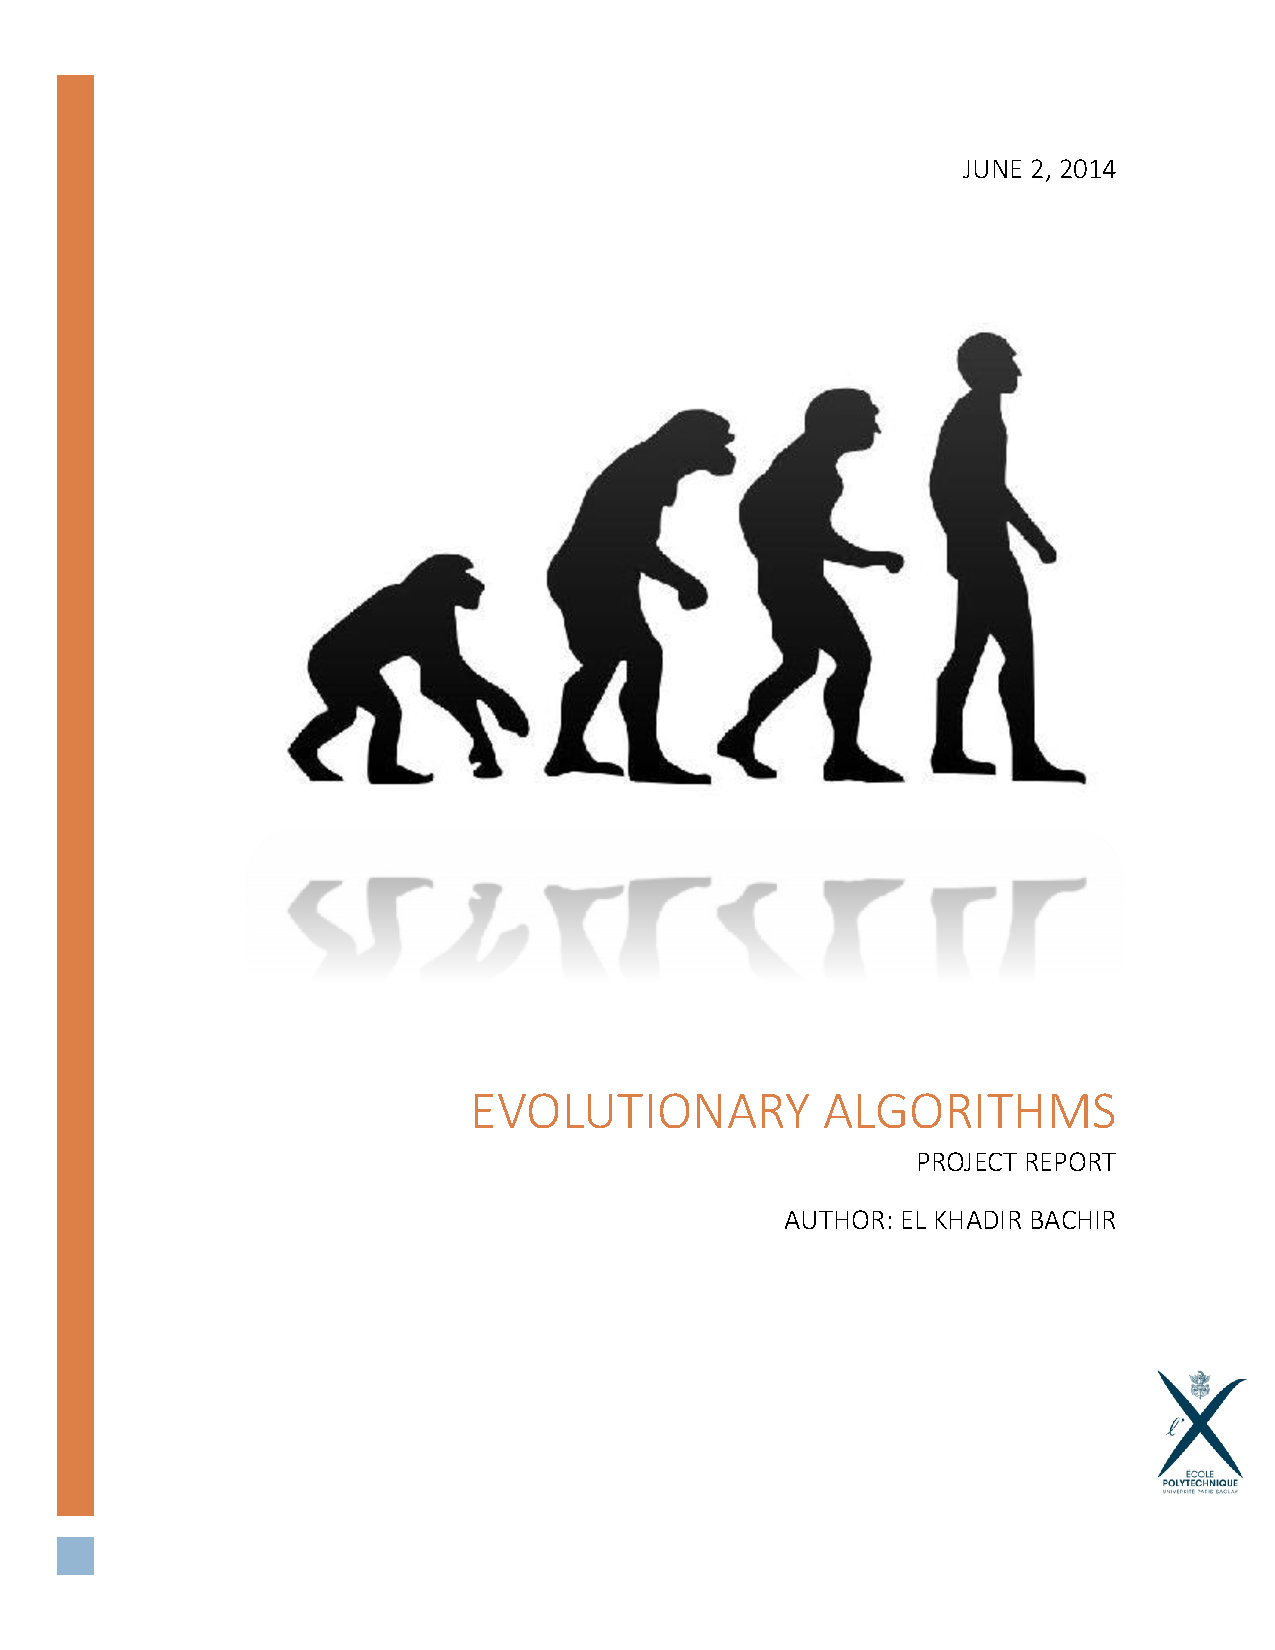
\includepdf{img/pagedegarde.pdf}


\begin{abstract}
This paper presents the results of the application of Evolutionary algorithms on various problems. The problems are different, but the modelling remane the same. The first section presents a generic class EA implementing the base mechanism of genetic algorithm. For each problem, we must find a suitable representation for the individuals (tuple, matrix ...), then we must implement a fitness function and a mutation/crossover operator.

I chose \textbf{Python} as a programming langage.

\textbf{Libraries used:}
\begin{itemize}
	\item numpy/scipy: provides powerful tools to manipulate arrays and generate random numbers
	\item pydot: allows to easily draw  graphs from Python
	\item pygame: for image rendering
	\item pyalgotrade: provides financial tools, used only in the last program
\end{itemize}
\end{abstract}

\tableofcontents

\section{Implementation of the GA algorithm (file "ga.py") }

The EA class implmenets the (self adapt) $(1+(\lambda, \lambda))$ GA in a generic form. The constructor is:
\begin{minted}{python}
 def __init__(self, fitness, mutation=default_mutation, crossover=default_crossover, 
                 l_distribution=np.random.binomial)
\end{minted}
It requires:
\begin{itemize}
	\item a fitness function to evaluate individuals,
	\item a mutation operator, by default, this operator is used:
\begin{minted}{python}
	def default_mutation(l, x):
		bits_to_change = random.sample(range(len(x)), l)
		x_mut = list(x)
		for b in bits_to_change:
			x_mut[b] = 1 - x_mut[b]
		return x_mut
\end{minted}
	\item a crossover operator
\begin{minted}{python}
	def default_crossover(c, x, xx):
		parent = [x, xx]
		parent_choice = bernoulli.rvs(c, size=len(x))
		return [ parent[p][i] for i, p in enumerate(parent_choice) ]
\end{minted}
	\item a function that generates $l$ from some distribution. By default, $l$ is generated from a binomial distribution.
\begin{minted}{python}
	def default_rule(offspring_size, better_solution_found):
		return offspring_size
\end{minted}
\end{itemize}

Then, the \textit{run} function does all the work. It generate the children, select the best one, does the crossover and mutation phase, adapt $\lambda$ if needed, and then repeat the process \textit{n generations} times.  

\begin{minted}{python}
def run(self, n, x_init, offspring_size=5, n_generations=10, 
				self_adapt_rule=default_rule, max_fitness=None )
\end{minted}

\begin{itemize}
	\item $n$ is the size of individuals
	\item $x\_init$ is the initial individual
	\item $offspring\_size$ is $\lambda$
	\item $n\_generations$ is the maximum number of generations before the function ends
	\item $self\_adapt\_rule$ is function that updates $\lambda$ in each loop. The default rule is the rule that does nothing:
\begin{minted}{python}
def default_rule(offspring_size, better_solution_found):
	return offspring_size
\end{minted}
	The $1/5^{th}$ rule would be:
\begin{minted}{python}
def one_fifth_rule(offspring_size, better_solution_found):
	F = 1.5
	if better_solution_found:
			return max(1, offspring_size / F)
	else:
			return offspring_size * (F**(0.25))
\end{minted}
	\item $max\_fitness$: when the fitness of $x$ is greater than $max_fitness$, the function returns immediately
\end{itemize}

\section{The One-Max problem  (file "onemax.py")}
The implmentation of the one-max problem is straight forward. 
We start with a random vector in $\{0, 1\}^n$. Default mutation and crossover operator work fine. 
For the fitness function, we sum all the bits in x (there is a builtin function \textit{sum} provided with \textit{Python}). The code is as follow:
\begin{minted}{python}
ea_algo = ga.EA(fitness=sum)
x_init 	= np.random.random_integers(0, 1, size=n)
best_x 	= ea_algo.run(n, x_init, offspring_size=5, n_generations=100)
\end{minted}

\Stats
All numbers reported are derived from $100$ independent runs of the respective algorithms. 
In all experiments reported below, we set $p = \frac{\lambda}{n}$ and $c = \frac{1}{\lambda}$.

For raw data, see "`onemaxstats.zip"'. Stat files contains data in the following format:\\
$n$  $\lambda $ \\
$N$ \\
$a_1$ $a_2$ ... $a_N$ \\
Where $a_i$ is the result obtained for the $i^{\text{th}}$ realisation.

\IMG{stat_onemax_1.png}{Number of fitness evaluations for $\lambda \in \{1, 4, 8, 12\}$}{0.5}

The $1+(8+8)$-EA gives the best results, better than the classic (1+1)-EA.

I tried the self-adaptive rule, that is:
$$ \lambda = \left\{
\begin{array}{l}
  \lambda / F \, \text{after a successful iteration} \\
  \lambda * F^{1/a} \, \text{otherwise}
\end{array}
\right.$$
with $a \in \{3, 4, 6, 9\}$
\IMG{stat_onemax_2.png}{Number of fitness evaluations for $a \in \{3, 4, 6, 9\}$}{0.5}
Whatever the initial value for $\lambda$, the self-adaptive version of the algorithm behave like the best version of the $1+(\lambda+\lambda)$-EA, that is $\lambda=8$.

\section{The Maximum Matching  (file "matching.py")}
We represent an undirected graph by it's adjacency list. For example:
\begin{minted}{python}
vertices = range(n)
edges = [(1, 2), (3, 4)]
\end{minted}

The function responsible for calculating the degree of a vertex $v$ in ine the subgraph consisting of the edges of $M$:
\begin{minted}{python}
def deg(M):
    deg_m = np.zeros(n)
    for i, (e, f) in enumerate(edges):
        if M[i]:
            deg_m[e] += 1
            deg_m[f] += 1
    return sum([max(0, d-1) for d in deg_m])
\end{minted}

And the fitness function:

\begin{minted}{python}
def fitness(M): 
    return sum(M) - m * deg(M)
\end{minted}


\Stats

For raw data see "`\textbf{matchingstats.zip}"'.

\subsubsection{First example: rings of size $n$}

\begin{tabular}{cc} 
	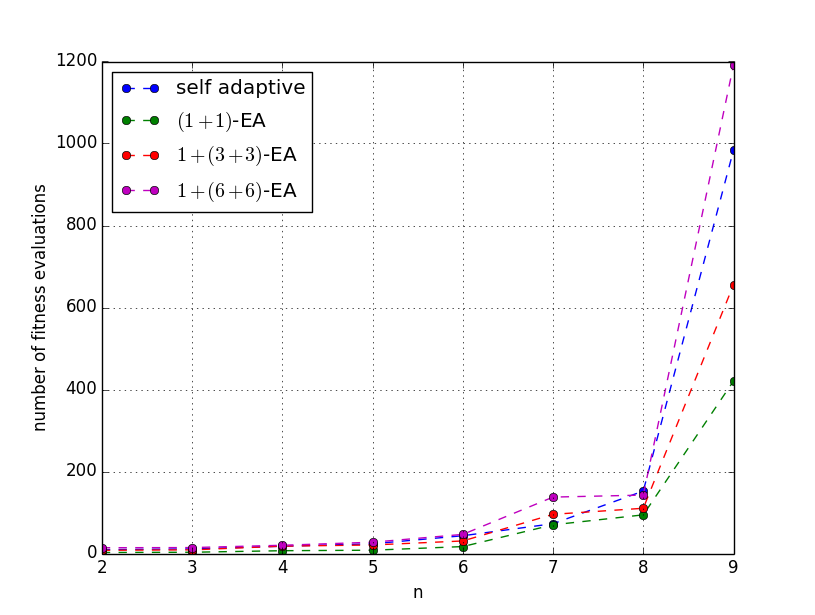
\includegraphics[scale=0.5]{img/stat_matching_1.png} & 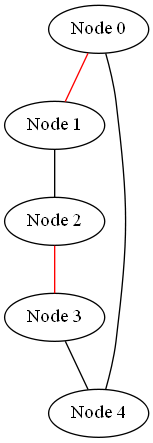
\includegraphics[scale=0.5]{img/max_graph.png} \\
	Number of fitness evaluations  & Instance
\end{tabular}

Unlike the onemax problem, the traditional $(1+1)-EA$ gives the best results.

\subsubsection{Second example: random graphs}
\textbf{Protocol}: We took $n=10$ fixed and $\lambda \in \{1, 3, 6\}$. I generated $N=1000$ independant random graph with $n$ vertices, Each of them chooses uniformly at random 3 friends. The following graph shows how the fitness evolves over time in average.


\begin{tabular}{cc} 
	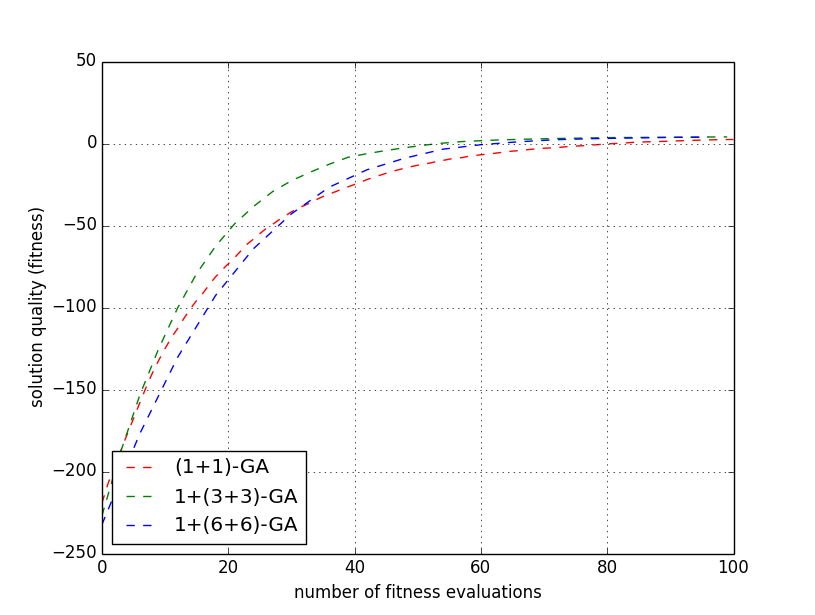
\includegraphics[scale=0.5]{img/random_graph_stat.png} & 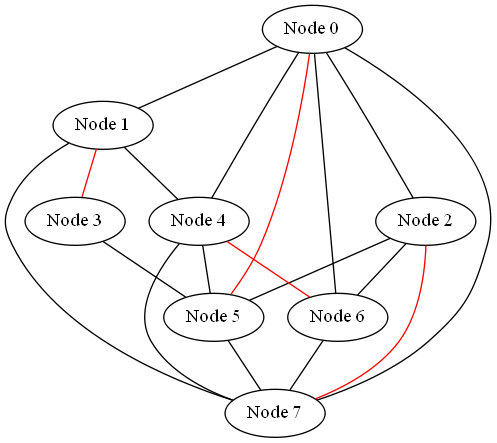
\includegraphics[scale=0.4]{img/random_graph_matching.png} \\
	Solution quality (fitness) evolution over time & Random instance
\end{tabular}

\section{Euler cycles (file "eulerian cycle.py")}
We represent graphes by their adjacency matrix. 

\textbf{Individuals} are represented by a list of matchings, ie $x = \{ M_v  \mid v  \in V \}$ where each $M_v$ is a dictionnary.

\textbf{Helper functions:}
\begin{minted}{python}

# Matches e and f
def match(Mv, e, f):
	Mv[e] = f
	Mv[f] = e
    
def find_match_and_remove(Mv, e):
	# Look for an edge f matched to e
	f = Mv.pop(e, None)
	# Remove the matching (if possible)
	if f is not None:
			del Mv[f]
	return f
		
def count_walks(x):
	# k is the number of independant paths induced by the matching x
	k = 0
	xx = deepcopy(x)
	# Each vertex v, we follow and remove the path induced by the matching
	for v in vertices:
		while len(xx[v]) > 0:
			e, f = xx[v].popitem()
			del xx[v][f]
			is_cycle = False
			# follow the path in both directions
			for i, j in [ (e, f), (f, e)]:
				# if we have found a cycle, there is no need
				# to follow the path in the opposite direction
				if is_cycle: break
				
				# s is the current vertex, i the precedent, and j the next
				# i -> s -> j
				i, s = v, j
				while j != None:
						j = find_match_and_remove(xx[s], i)
						i, s = s, j
				# we have found a cycle if the last vertex visited == v
				is_cycle = (i == v)    
				k += 1
	return k
\end{minted}

We can use the default \textbf{crossover} operator.

We implement the \textbf{mutation} operator as suggested:
\begin{minted}{python}
def mutation(l, x):
	x_mut = deepcopy(x)
	for _ in range(l):  
		# Choose a random vertex v
		v = random.randint(0, n-1)
		Mv = x_mut[v]
		deg_v = sum([edges[v][i] for i in vertices if i != v])
		if deg_v < 2:
			raise Exception('The graph is not eulerian because 
			vertex %d has deg = %d' % (v, deg_v))
		# if deg(v) == 2, a trivial perfect matching is [ (i, j) ]
		elif deg_v == 2:
			i, j = [w for w in vertices if edges[v][w] and v != w]
			match(Mv, i, j)
		else:
			# Choose a random edge e incident to v, 
			e = random.choice([i for i in vertices if i != v and edges[v][i]])
			# See if it is matched. If it's the case, remove the match
			f = find_match_and_remove(Mv, e)
			
			# Same thing for (ee, ff)
			ee = random.choice([i for i in vertices if (not i in[ v, e, f]) and edges[v][i]])
			ff = find_match_and_remove(Mv, ee)
			
			# match (e, ee) and (f, ff) if possible
			match(Mv, e, ee)
			if f and ff:
				match(Mv, f, ff)
							
	return x_mut
\end{minted}

The fitness function:
\begin{minted}{python}
def fitness(x):
	k = count_walks(x)
	cycles_penality = nb_edges - sum(map(lambda Mv: len(Mv), x))/2  
	return  - cycles_penality  - (k-1)
\end{minted}

We run the program as follow:
\begin{minted}{python}
def poisson_distribution(n, p):
    return 1 + np.random.poisson(1)  
		
# Start with empty matchings
x_init = [ {} for _ in range(n)]
best_x = ea_algo.run(n, x_init=x_init, offspring_size=4, n_generations=1000, 
				max_fitness=0, l_distribution=poisson_distribution)
\end{minted}


After the algorithm has finished, we can reconstruct the tour from the maximum matching:

\begin{minted}{python}
# Reconstruct the tour induced by x
def reconstruct_tour(x, start=0):
    xx = deepcopy(x)
    if len(xx[start]) == 0: return []
    
    # v is the current vertex, i the precedent, and j the next
    # i -> v -> j
    i, j = xx[start].popitem()
    path = [i, start, j]
    i, v = start, j
    while j is not None:
        j = find_match_and_remove(xx[v], i)
        path.append(j)
        i, v = v, j
    return path[:-1]  
\end{minted}

\subsection{Some Tests}

See the file "graph.py" for graph creation and rendering.

\begin{tabular}{cc} 
	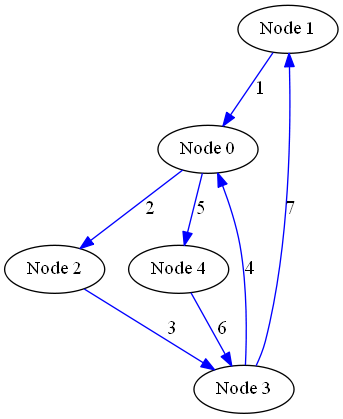
\includegraphics[scale=0.5]{img/random_graph_cycle.png} & 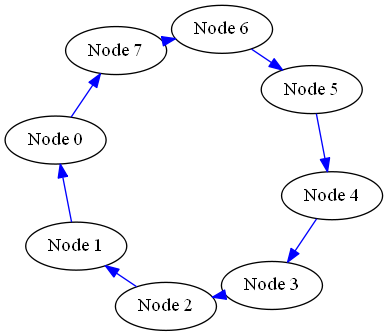
\includegraphics[scale=0.5]{img/ring_graph_cycle.png} \\
	\multicolumn{2}{c}{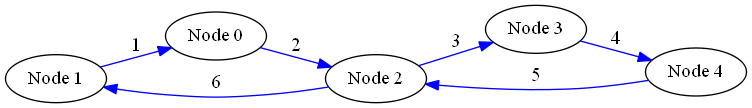
\includegraphics[scale=0.5]{img/triangle_graph_cycle.png}} \\
	\multicolumn{2}{c}{Example of tours found by the algorithm}
\end{tabular}

For the following simulations, I compare the average optimization time of the $(1+(\lambda, \lambda))$ GA for $l$ following the $B(n, p)$ distribution and $P(1)$ distribution. As graph instance, I took triangular graphs: \\
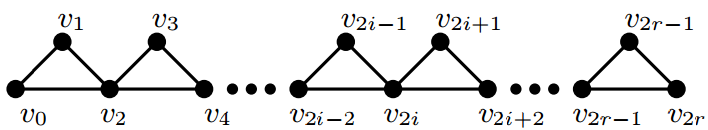
\includegraphics{img/triangle_graph.png} 

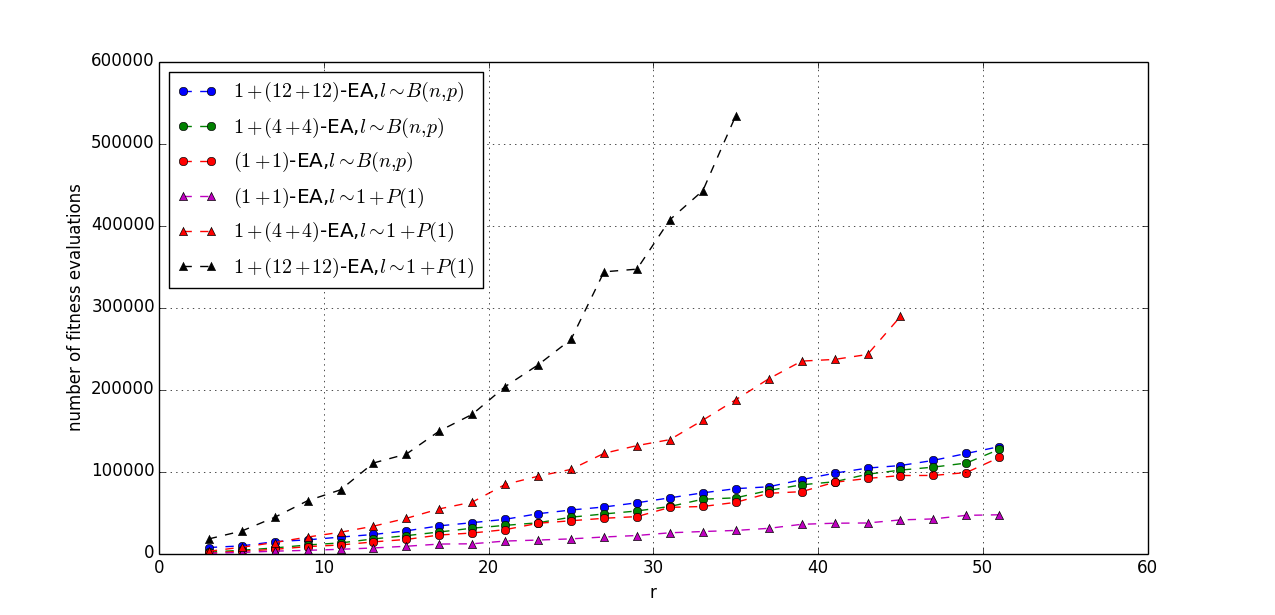
\includegraphics[scale=0.5]{img/stat_euler.png} 

when $l$ follows a binomial distribution, the performance is independant from the value of $\lambda$. 
When $l$ follows a poisson distribution, it's better to choose $\lambda=1$.

For raw data, see "eulerstats.zip".

\section{Own Idea}

\subsection{The N-Queen's Problem  (file "chess.py")}
In chess, a queen can move  horizontally, vertically, or diagonally. Given a chess board with $N$ rows and $N$ columns, N-Queen's problem asks how to place N queens on the chess board so that none of them can hit any other in one move.


Since the number of queens is equal to the number of rows/columns, in each row there is exactly one queen, and two different queens are placed in two different columns. Therefore a configuration (position of the queens on the chess board) is represented with a permutation of $\{0, ..., N-1\}$.
An individual is a N-tuple $x = (x_1, ..., x_N)$, where $0 \leq x_i < N$  is the column of the queen placed on the row $i$. We start with the N-tuple $(0, ..., N-1)$: \mint{python}|x_init = range(n)|


With this representation, there will be no queens on the same row/column. We only have to check for possible collisions diagonally. The \textbf{fitness} function counts the number of those collisions: 
\begin{minted}{python}
def fitness(t): 
	x = np.zeros((n , n))
	for i, j in enumerate(t):
		x[i][j] = 1

	s = 0
	# diags
	for k in range(-n + 1, n):
		# diag (i, i+k) (n-i-1, i+k)
		q_diag = sum([ x[i][i + k] for i in range(max(0, -k), min(n, n - k))])
		s += max(0, q_diag - 1) 
		q_diag = sum([ x[n - i - 1][i + k] for i in range(max(0, -k), min(n, n - k))])
		s += max(0, q_diag - 1)
	return -s 
\end{minted}

The \textbf{mutation} operator select $l$ random elements, and permutates them randomly:
\begin{minted}{python}
def mutation(l, x):
	# selection of the bits to mutate
	bits_to_change = random.sample(range(len(x)), l)
	
	# apply a random permutation to bits_to_change
	rand_permutation = list(bits_to_change)
	random.shuffle(rand_permutation)

	x_mut = list(x)
	
	for i in range(l):
		x_mut[bits_to_change[i]] = x[rand_permutation[i]]
		
	return x_mut
\end{minted}

The \textbf{crossover} operator select a parent $p$: $x$ with probabilty $c$ and $xx$ with probability $1-c$. Then it find an element that is not already present in the child $y$, add it to y, and then repeat $n$ times:
\begin{minted}{python}
def crossover(c, x, xx):
	parent = [x, xx]
	parent_choice = bernoulli.rvs(c, size=len(x))
	y = []
	for p in parent_choice:
		# Avoids repeating the same number in the permutation y
		for b in parent[p]:
			if not (b in y):
				y.append(b)
				break
	return y
\end{minted}

\IMG{queen.png}{A Valid configuration}{0.4}

(see the file "draw.py" for drawing function)

\subsection{2D Image reconstruction  (file "2d reconstruct.py")}
This program tries to rebuild a 2D grey scale image using only disks. Individuals are strings representing a list of 256 circles $\{ (x, y, radius, color, alpha) \}$ in binary format where:
\begin{itemize}
	\item $x$ and $y$ are the position of the center of the circle
	\item $color$ is an integer between $0$ and $255$ giving the tone of grey the circle must be filled with
	\item $alpha$ is the transparency
\end{itemize}


The fitness function is a per-pixel RGB comparison:

\begin{minted}{python}
def fitness(x):
	draw_spheres(x)
	pixels = array2d(srf)
	return -np.linalg.norm((reference_pixels - pixels) / M)
\end{minted}

Since we use a string based representation, we can use the default crossover and mutation operators as in the first algorithm.

Here is the result:
\IMG{source.jpg}{Source image}{0.75}

\IMG{evolution.png}{Evolution}{0.75}


\subsection{Finance (file "finance.py")}
Genetic algorithm can be used in trading. Trading strategies (individuals) can be represented by boolean trees, for instance:
\IMG{trading_strategy.png}{A tree representing a trading strategy}{0.75}

It can be interpreted as a boolean value like this: 
If:
\begin{itemize}
	\item the average of the 50 last stock values is less the actual price
and the min of the 6 last stock values is less the actual price. then answer True, else False
\end{itemize}
If the answer is True, then send a BUY signal, and SELL signal otherwise.

See the file \textbf{"`rules.py"'} for the tree representaion.

\begin{itemize}
	\item The fitness is the benefit we gain if we apply this strategy daily during a year to a given share (ORACLE for example). I use the library \textbf{pyalgotrade} to calculate the fitness.
	\item The mutation operator changes some random nodes of the tree.
	\item The crossover operator takes a sub tree of $x$ and replace it by a sub tree of $xx$.
\end{itemize}

The output of the program is a tree like this:
\IMG{best_strategy.png}{Best trading strategy}{0.4}
This strategy has a fitness of 76\$.

\end{document}
